\documentclass{article}
\title{\vspace*{\fill}\textbf{Peer-to-Peer Chat Application}}
\author{Agam Agarwal (CS12B1003)\\
		Sachin Jaiswal (CS12B1033)\\
		Adarsh Pugalia (ES12B1001)}

\usepackage{listings}
\usepackage{array}
\usepackage{tikz}
\usetikzlibrary{arrows, positioning}

\begin{document}
	
	\maketitle
	\vspace*{\fill}

	\newpage
	\tableofcontents
	
	\newpage

	\section{Introduction}
	We developed a terminal-based chat application which works on a peer-to-peer model. There is a server which maintains a list of currently online clients, while the clients can chat with each other directly. The transport layer protocol used is \textbf{UDP (User Datagram Protocol)}.

	The model of the application is as follows:\\\\\\
	
	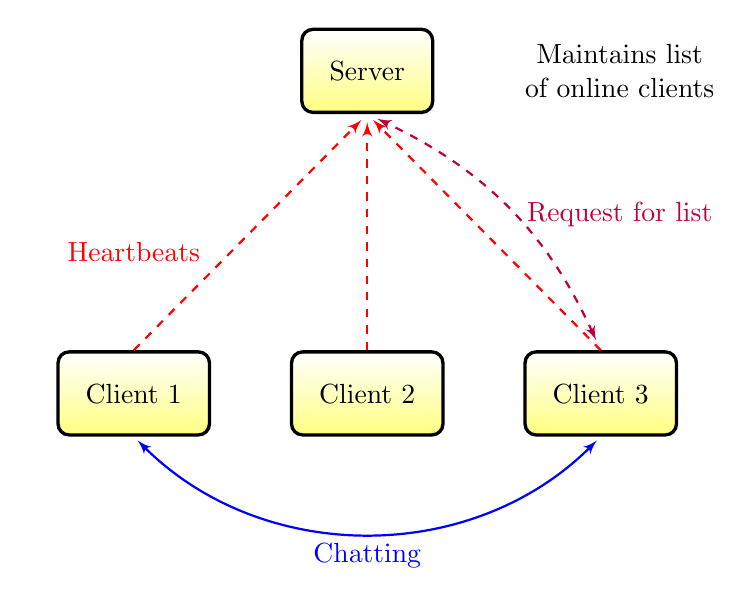
\begin{tikzpicture}
		\tikzset{
			host/.style={rectangle, rounded corners, draw=black, top color=white, bottom color=yellow!50,very thick, inner sep=1em, minimum size=3em, text centered},
			heartbeat/.style={->, >=latex', color=red, shorten >=3pt, thick, dashed},
			label/.style={text width=7em, text centered},
			chat/.style={<->, >=latex', color=blue, shorten >=2pt, shorten <=2pt, bend right=45, thick},
			listrequest/.style={<->, >=latex', color=purple, shorten >=4pt, shorten <=4pt, bend right=20, thick, dashed}
		}
		\node[host] (server) {Server};
		\node[host, below=3cm of server] (client2) {Client 2};
		\node[host, left=of client2] (client1) {Client 1};
		\node[host, right=of client2] (client3) {Client 3};

		\node[label, right=of server] (servertask) {Maintains list of online clients};
		\node[label, above=of client1, color=red] (heartbeat) {Heartbeats};
		\node[label, below right=of server, color=purple] (list) {Request for list};

		\draw[heartbeat] (client1.north) to (server.south);
		\draw[heartbeat] (client2.north) to (server.south);
		\draw[heartbeat] (client3.north) to (server.south);

		\draw[listrequest] (client3.north) to (server.south);
		\draw[chat] (client1.south) to node[auto, swap] {Chatting}(client3.south);
	\end{tikzpicture}

	\newpage
	\section{How to use the application}
	The chat application has two parts as stated above: Server and Client
	
	\subsection{Server}
	The main class of the server can be run using the following command:
	\begin{lstlisting}[language=bash]
	java in.ac.iith.chat.server.ServerMain
	\end{lstlisting}
	Alternatively, you can start the server using the executable jar file attached, with the following command:
	\begin{lstlisting}[language=bash]
	java -jar Server.jar
	\end{lstlisting}
	The server will launch in the terminal and will continue to run indefinitely. In order to stop the server, use the following command:
	\begin{lstlisting}
	exit
	\end{lstlisting}
	The server will print a message whenever a new client joins, or is removed.


	\subsection{Client}
	The main class of the client can be run using the following command:
	\begin{lstlisting}[language=bash]
	java in.ac.iith.chat.client.ClientMain [server_address]
	\end{lstlisting}
	Alternatively, you can start the server using the executable jar file attached, with the following command:
	\begin{lstlisting}[language=bash]
	java -jar Client.jar [server_address]
	\end{lstlisting}
	In both the above commands, the `server\_address' is an optional argument.

	When the client program starts, it prompts the user for server address(in case not given as a command line argument) and a unique nickname. If the nickname is already taken, the user is prompted again. The nickname can contain letters and digits only.

	Once the connection is established, the user can start interacting with the program using the following commands.

	\begin{center}
		\begin{tabular}{ >{\bfseries}c c l }
			help & - & Display a help text with information about all commands \\\\
			l & - & Get the latest list of online clients from the server \\\\
			c & - & Connect to one of the online clients. Format `c [nickname]' \\\\
			m & - & Send a message to the current chat partner \\\\
			bye & - & Disconnect from the current chat partner \\\\
			exit & - & Exit the client program
		\end{tabular}
	\end{center}

	\newpage
	\section{Working}
	The server has a single UDP socket open. It uses this socket to communicate with the clients. Each of the clients have two UDP sockets open. One is used for communicating with the server, while the other is used for communicating with other clients. Each of the clients sends a \textbf{heartbeat} to the server at regular intervals\footnote{current value=1 second}. Along with the heartbeat, the client sends information about its nickname(\textit{unique}) and the port on which it is listening to the other clients.\\

	The server uses a \textbf{HashMap} to maintain a list of online clients. In this map, it stores the \textbf{time-stamp} of the last heartbeat it received from the client, its nickname, IP address, and the port on which it is listening to other clients.
	At regular intervals\footnote{current value=1 second}, the server iterates through the list of clients to see which clients have expired\footnote{current value of expire time=5 seconds}, and removes these clients from the hash map.\\

	A client may request the server for the list of online clients. The server replies with a properly formatted list of online clients. The client maintains a copy of this list at its end. The client may send a request to connect to another client by using its nickname. If the other client accepts this request, they both can start sending messages to each other. If the other client doesn't respond, the request is timed out\footnote{current value=10 seconds} and considered as `denied'.Anyone of them may end the chat by typing `bye'.
	If two clients are chatting with each other, and a third client tries to connect to one of them, its request is automatically rejected.\\

	Both the server-client communication and client-client communication are implemented using UDP. The reason for this is that a client just needs to send a small heartbeat packet to the server. The server would reply with a simple `accept' or `reject' message for the first heartbeat sent. The other type of communication between the client and the server is the query for the list. Even if either of the packets(request or reply) is lost, the client program displays the last updated list of clients. On the other hand, the server allows a sufficient amount of time before deciding that the client went offline, this would avoid the issues due to lost heartbeat packets. Moreover, by using UDP, the server doesn't need to open different sockets for communicating with different clients, it can listen to all the clients on the same UDP socket.\\

	In the client-client communication, the reason behind using UDP was that chat messages are usually short and real-time messages. UDP doesn't have the overhead of connection and reconnection(in case the connection is lost in between) which TCP has, and thus is faster. The order of messages doesn't need to be strictly preserved during real-time chatting, therefore using TCP instead of UDP doesn't give much gains.
\end{document}
